\documentclass[11pt,a4paper]{article}
\usepackage{graphicx}
\usepackage[utf8x]{inputenc}
\usepackage[T1]{fontenc}
\usepackage{blindtext}
\usepackage{enumitem}
\usepackage{hyperref}
\usepackage{multirow}
\usepackage{pdflscape}
\usepackage{afterpage}
\usepackage{capt-of}% or use the larger `caption` package
\usepackage{lipsum}% dummy text
\usepackage[table]{xcolor}% http://ctan.org/pkg/xcolor
\usepackage[toc,page]{appendix}
\usepackage{float}

\setcounter{secnumdepth}{5}
\setcounter{tocdepth}{5}

\begin{document}

\begin{titlepage}
	\centering
	{\scshape\LARGE Universidade de Brasília - Faculdade Gama\par}
	\vspace{1cm}
	{\scshape\Large Modelagem de Processos\par}
	\vspace{1.5cm}
	{\huge\bfseries Proposta de modelagem para suporte ao usuário\par}
	\vspace{2cm}
	{\Large\itshape João Henrique Pereira de Almeida\par}
	\vfill
	%supervised by\par
	%Dr.~Mark \textsc{Brown}

	\vfill

% Bottom of the page
	{\large \today\par}
\end{titlepage}


\tableofcontents
\listoffigures
\listoftables

\clearpage
\section{Informações de contexto}

\subsection{Contexto}
	O cenário desse trabalho é o de uma empresa que
	fornece uma solução completa, composta por hardware e software.
	Essa solução tem como objetivo a emissão de cupons fiscais que são emitidos no
	caixa de supermercados durante a compra.
	O produto de software é responsável por identificar o item quando passados no
	identificador de código de barras. A solução de hardware é composta pelo identificador
	de código de barras, e o emissor de cupom fiscal. Como a empresa em questão é
	provedora de dois items, o serviço de atendimento ao
	usuário se faz necessário pois tais soluções podem apresentar algum defeito, ou
	o usuário não conseguir ter uma experiência de uso desejada.
	O público alvo dessa empresa são supermercados ou quaisquer empreendimento
	que busca ter catalogados seus items, e disponibilizar para venda. O contexto
	abordará somente o atendimento do usuário(supermercados) em relação ao uso das duas soluções.
	O processo de suporte aos usuários das soluções se encontra disforme e não vem obtendo
	os resultatos (relatos) esperados, causando insatisfação dos clientes, além de gastos por parte da empresa.
	Devido a esses problemas os usuários(supermercados) deixam de lucrar, agravando ainda mais a insatisfação
	dos clientes. Buscando resolver esse problema e ainda agregar valor para o usuário provendo
	um serviço eficiente e eficaz.
	\\A empresa solicitou que seu nome não fosse citado nos resultados aqui mostrados, esse pedido
	se fez necessário pois a mesma está sobre o processo de direito de imagem e venda.

\begin{flushleft}
\section{Informações Adicionais}

\subsection{Motivação}
Quando se pensa sobre os principais fatores que colaboram para o sucesso de
empresas a  satisfação do cliente no mercado de TI exerce um papel importante,
e \textit{user experience} é com certeza um dos principais fatores, os caminhos
para prover a \textit{user experience} são muitos, por exemplo prover qualidade
no serviço de usuário, pode ser um desses caminhos. Consequentemente vemos o
suporte ao usuário como sendo um serviço provido por uma empresa  ao seus
clientes com o objetivo de melhorar a experiência com o produto provido. Em
outras palavras o serviço de suporte ao usuário ajuda ao cliente resolver
qualquer problema que possa encontrar enquanto usa o produto ou serviço

\end{flushleft}

\subsubsection{Serviço de suporte ao usuário}
Primeiramente devemos definir o que é o serviço de suporte na área de TI,
podemos encontrar vários termos como:
\begin{itemize}[noitemsep]
  \item Suporte tecnico;
  \item Service Desk;
  \item Help Desk;
  \item Suporte ao Cliente;
  \item Suporte;
  \item Suporte ao usuário;
  \item Etc.
\end{itemize}

Basicamente esses termos definem a mesma coisa, mas cada um deles é focado
em diferentes aspectos do serviço, então para isso vamos focar no suporte
ao usuário, pois esse é mais comum e com isso evitamos ambiguidades.
Logo entende-se como suporte ao usuário um serviço provido por uma organização
para seus clientes para promover uma experiência com seu produto ou serviço,
resolvendo qualquer problema que o cliente possa encontrar enquanto usa o
serviço ou produto. Além disso não se  deve colocar qualquer restrição ao tipo
de problema que possa ser encontrado ou qualquer dúvida ou denuncia que o
cliente possa reportar.

\section{Execução do Projeto}
\subsection{Fase 1 - Análise}
\begin{itemize}[noitemsep]
	\item Compreensão do contexto
	\item Definir o problema
	\item Definir dos objetivos
	\item Formalizar os processos correntes (AS-IS)
	\item Identificar os envolvidos
	\item Análise das informações
\end{itemize}
\subsection{Fase 2 - Otimização}
\begin{itemize}[noitemsep]
	\item Definir os Fatores de Sucesso
	\item Otimização dos processos identificados (TO-BE)
	\item Documentação de novos processos
\end{itemize}
\subsection{Fase 3 - Implantação}
\begin{itemize}[noitemsep]
	\item  Implantação dos novos processos
\end{itemize}

\subsection{Fase 4 - Validação}
\begin{itemize}[noitemsep]
	\item Implantação do processo de monitoramento
\end{itemize}

\section{Definição do Problema}

\begin{figure}[!h]
\caption{Descrição de problemas pelos envolvidos}
\centering % para centralizarmos a figura
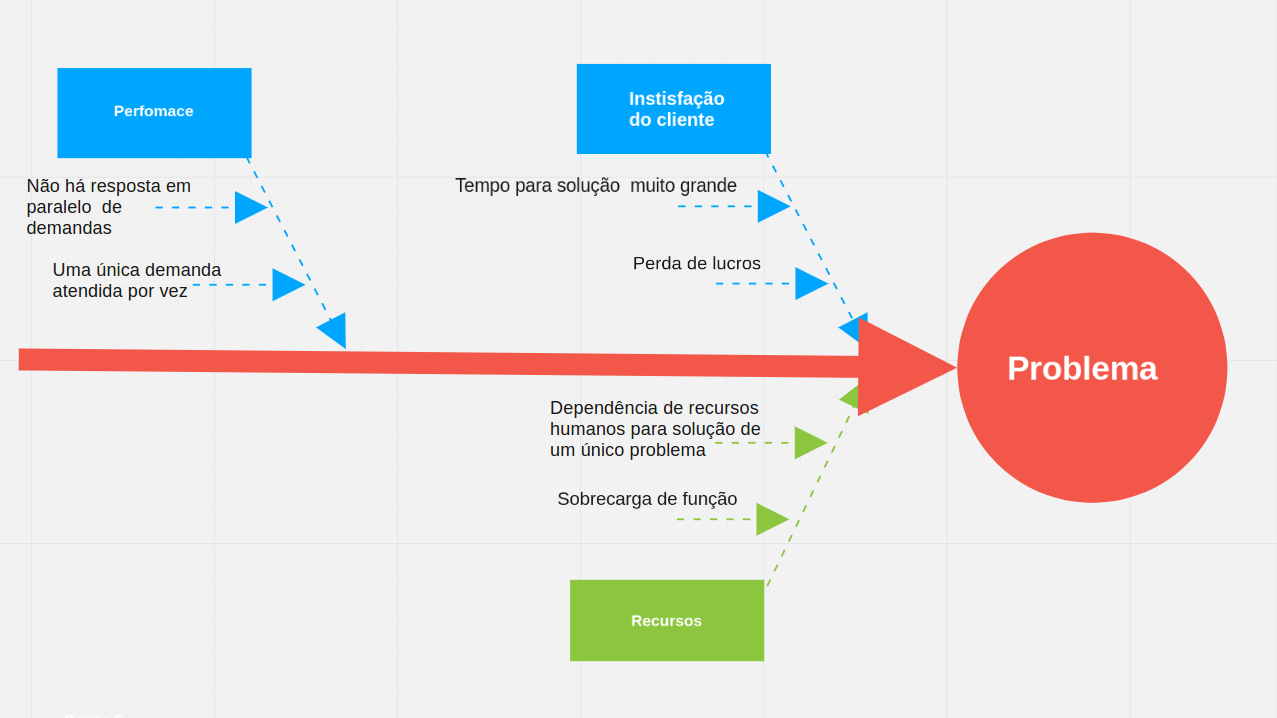
\includegraphics[width=15cm]{fishbone.png}
\label{figura:Fishbone de Problemas }
\end{figure}


\begin{itemize}[noitemsep]
  \item Problema:
    \begin{itemize}
      \item O processo de suporte ao usuário é demorado, e demanda de muitos recursos
           humanos para que seja executado.
    \end{itemize}
  \item O problema afeta:
    \begin{itemize}
      \item Os clientes
    \end{itemize}
  \item Cujo impacto é:
    \begin{itemize}
      \item	O cliente que tem a demora da solucão do seu problema
           deixa de lucrar, pois o equipamento normalmente fica sem uso.
    \end{itemize}
  \item Uma solução bem sucedida seria:
    \begin{itemize}
      \item Uma boa solução seria um conjunto de atividades, que simplifique
       automatize algumas atividades desse processo.
     \end{itemize}
\end{itemize}

\subsubsection{Objetivos}
\begin{itemize}[noitemsep]
 \item Aumentar a satifsfação do cliente
 \item Formalizar o processo atual
 \item Diminuir a necessidade de tarefas humanas no processo de suporte
 \item Diminuição do tempo de processamento de uma requisição individual
 \item Projetar e implementar a sistema de monitoramento de perfomace
 \item Encontrar gargalos
\end{itemize}

\subsubsection{Principais indicadores}
\begin{itemize}[noitemsep]
 \item Avaliação dos usuários do sistema de suporte
 \item Tempo médio gasto para a realização de um atendimento
 \item Quantidade de recurso humano gasto nesta macroatividade
\end{itemize}

\subsubsection{Envolvidos}
\begin{itemize}[noitemsep]
 \item Operador de suporte
 \item Desenvolvedor Sênior
 \item Representante de Vendas
 \item Chefe de tecnologia
\end{itemize}

\section{Modelo AS-IS}

\subsection{Modelos dos processos}
Nessa seção vamos abordar a modelagem dos processos identificados no contexto,
os processos aqui mostrados usam a notação do BPMN para dar clareza e objetividade.
Proporcionando um padrão internacional de leitura dos mesmos.

\subsubsection{Gerência de requisição}
\begin{figure}[!h]
\caption{Gerencia de requisição}
\centering % para centralizarmos a figura
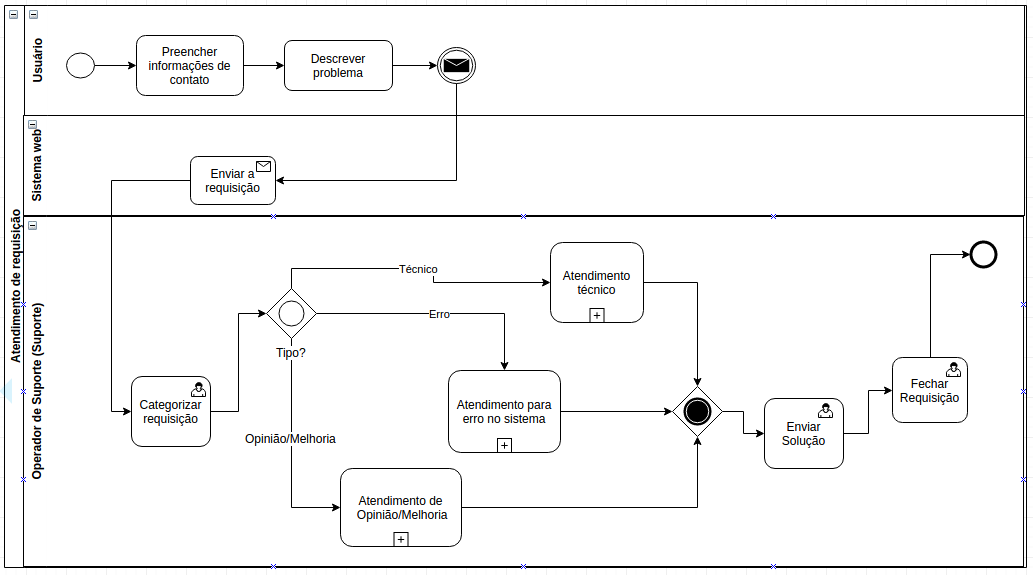
\includegraphics[width=15cm]{as-is/01_atendimento_de_requisicao.png}
\label{figura:atendimento_requisicao_as_is}
\end{figure}

\begin{itemize}[noitemsep]
	\item Preencher informações de contato
		\begin{itemize}
			\item O usuário preenche um formulário com o nome, email e telefone de contato
		\end{itemize}
	\item Descrever problema
		\begin{itemize}
			\item Realiza a descrição do problema
		\end{itemize}
	\item Enviar requisição
		\begin{itemize}
			\item O sistema web envia um email para o operador
		\end{itemize}
	\item Categorizar requisição
		\begin{itemize}
			\item Atribui uma categoria correta a requisição
		\end{itemize}
	\item Enviar Solicitação
		\begin{itemize}
			\item Envia informação sobre a decisão/solução
		\end{itemize}
	\item Fechar requisição
		\begin{itemize}
			\item Marca como finalizada a requisição
		\end{itemize}
\end{itemize}


\subsubsection{Atendimento técnico}

\begin{figure}[!h]
\caption{Atendimento técnico}
\centering % para centralizarmos a figura
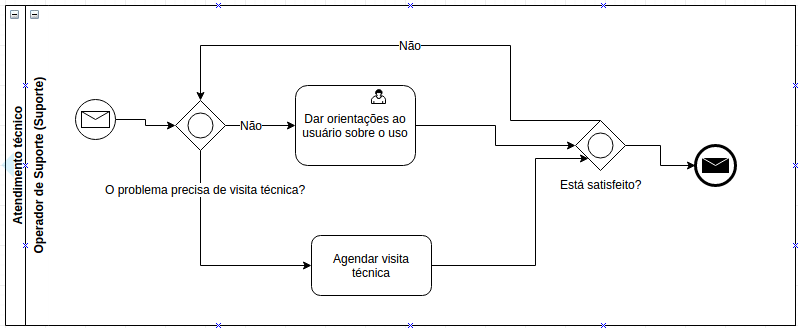
\includegraphics[width=15cm]{as-is/02_atendimento_tecnico.png}
\label{figura:suporte_tecnico_as_is}
\end{figure}

\begin{itemize}[noitemsep]
	\item Dar orientações ao usuário sobre o uso
		\begin{itemize}
			\item Dar orientações para que o usuário possa resolver um problema de uso
		\end{itemize}
	\item Agendar visita técnica
		\begin{itemize}
			\item Marcar data para a realização de uma visita
		\end{itemize}
\end{itemize}

\subsubsection{Atendimento para erro no sistema}
\begin{figure}[!h]
\caption{Atendimento para erro no sistema}
\centering % para centralizarmos a figura
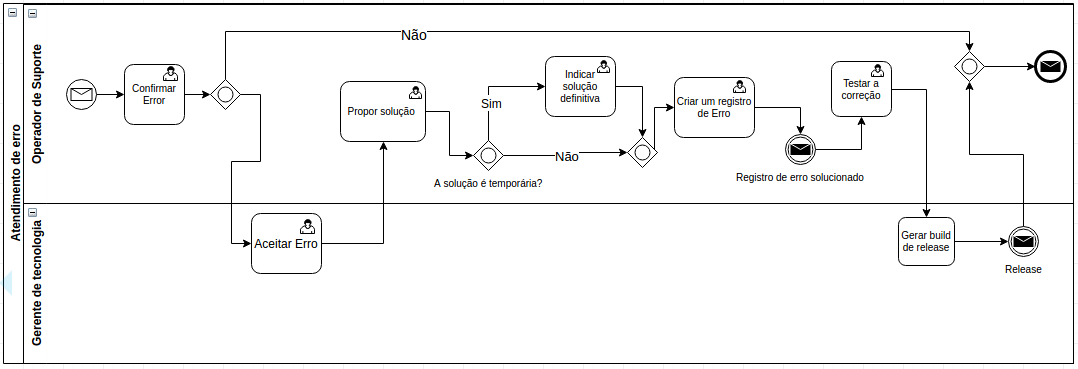
\includegraphics[width=16cm, height=5cm]{as-is/03_atendimento_de_erro.png}
\label{figura:atendimento_de_erro_as_is}
\end{figure}

\begin{itemize}[noitemsep]
	\item Confirmar erro
		\begin{itemize}
			\item Confirma se o erro realmente existe
		\end{itemize}
	\item Aceitar Erro
		\begin{itemize}
			\item Aceita a existência do erro e planeja a correção
		\end{itemize}
	\item Propor Solução
		\begin{itemize}
			\item E discutida uma solução, para ser implantada rapidamente
		\end{itemize}
	\item Indicar Solução definitiva
		\begin{itemize}
			\item Indica a melhor solução para o problema
		\end{itemize}
	\item Criar registro
		\begin{itemize}
			\item E registrado o erro solucionado
		\end{itemize}
	\item Testar correção
		\begin{itemize}
			\item E realizado testes que comprovem a correção do erro
		\end{itemize}
	\item Gerar build de release
		\begin{itemize}
			\item E disponibilizado para os clientes a versão atualizada
		\end{itemize}
\end{itemize}
\clearpage
\subsubsection{Atendimento de Opinião/Melhoria}

\begin{figure}[!h]
\caption{Atendimento de Opinião/Melhoria}
\centering % para centralizarmos a figura
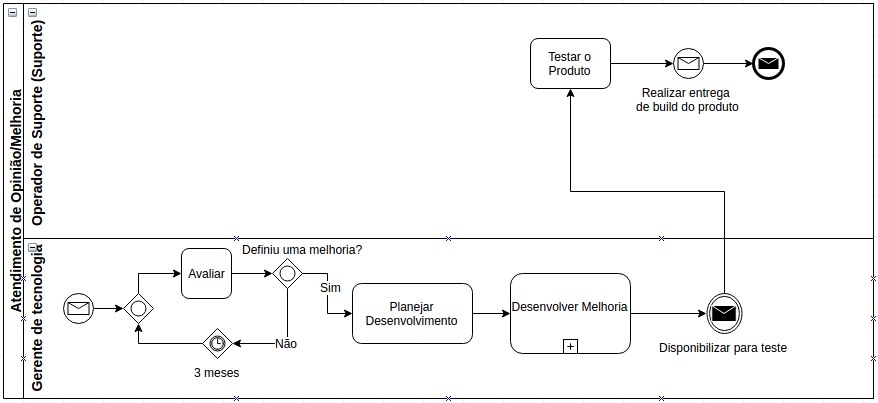
\includegraphics[width=15cm]{as-is/04_atendimento_de_melhoria.png}
\label{figura:atendimento_de_melhoria_as_is}
\end{figure}

\begin{itemize}[noitemsep]
	\item Avaliar
		\begin{itemize}
			\item Avaliar a proposta
		\end{itemize}
	\item Planejar Desenvolvimento
		\begin{itemize}
			\item E planejado o desenvolvimento da melhoria
		\end{itemize}
	\item Testar o produto
			\begin{itemize}
				\item E realizado testes que comprovem a adição da melhoria
			\end{itemize}
\end{itemize}


\subsection{Conclusão e análise - AS-IS}
\begin{itemize}[noitemsep]
  \item Processos indefinidos
  \item Ausência de monitoramentos
  \item Ausência de autenticação de usuário
  \item Processos de longo tempo de execução
  \item Reporte insuficiênte para o cliente
\end{itemize}

\section{Padrões e Normas}
\subsection{ITIL}

A ITIL define serviço como um meio intangível de entregar valor aos clientes,
facilitando resultados sem ter que assumir custos e riscos extras.E a ITIL mapeia
todo o ciclo de vida dos serviços através de 5 pilares\cite{itsmfservice}:
\begin{itemize}[noitemsep]
  \item Estratégia do Serviço
  \item Desenho de Serviço
  \item Transição de Serviço
  \item Operação do Serviço
  \item Melhoria Continuada
\end{itemize}

Estratégia do Serviço (“Service Strategy”): É aqui que são tomadas as deciões
estratégicas relacionadas aos serviços que vão ser desenvolvidos. Serviços que
ajudam na identificação de requisitos e outras necessidades que ajudam a
alcançar os objetivos do negócio.

Desenho de Serviço (“Service Design”): Basicamente desenha o que a estratégia
decidiu, tendo em mente os fatores de utilidade e garantia, tomando por base
as características esperadas para os serviços e culminando na elaboração e
descrição de especificações dos serviços.

Transição de Serviço (“Service Transition”): Tem por foco o gerenciamento de
mudanças, prevendo para tal fim a condução de ações voltadas à implantação de
serviços. Move os serviços para o ambiente de produção. Os serviços são
desenvolvidos, testados e liberados de forma controlada.

Operação do Serviço (“Service Operation”): Aqui estão os processos do dia-a-dia,
 que mantém os serviços funcionando assegurando que seus objetivos sejam
 alcançados, baseando-se para isto, em acordos de níveis de serviços
 (SLAs, sigla do inglês “Service-level Agreements”).

Melhoria Contínua do Serviço (“Continual Service Improvement”): Busca
constante pela evolução dos serviços, aplicando para isto conceitos
oriundos de técnicas como o ciclo PDCA (sigla do inglês “Plan-Do-Check-Act”).

Esses pilares, se destrinchados, nos fornecem um total de 26 processos e 4
funções, aprofundando o conceito de como estruturar um serviço de acordo com
áreas, fases do ciclo de vida e funções.



As práticas de ITIL procuram fornecer o suporte necessário para
que tais serviços estejam em sintonia com as necessidades do
negócio\cite{cartlidge2007introductory}. Dentre os benefícios que podem ser
obtidos a parte da utilização das técnicas que compõem ITIL, pode-se destacar:


\begin{itemize}[noitemsep]
	\item Melhorias na satisfação dos clientes/áreas dependentes de um ou mais serviços;
	\item Maior eficiência operacional;
	\item Redução nos custos e nos esforços desprendidos pela área de TI
    cumprimento de uma ampla gama de atividades;
\end{itemize}

Foi escolhida a utilização do ITIL versão 3, denominada
V3, por ser um framework aberto e bastante aceito na comunidade. Esta versão é
composta por cinco livros, onde cada um deles está relacionado a um estágio do
ciclo de vida do serviço. Na realização deste trabalho houve o foco apenas no
estágio que trata do serviço, isto é, o “Service Operation”;\\

\subsubsection{Operação de Serviço}
Operação de serviço é o mais relevante para suporte ao usuário
O propósito da Operação de Serviços é coordenar e realizar as atividades e processos q
requeridos para entregar e gerenciar os serviços em níveis acordados com usuários e
clientes. Enquanto as fases anteriores englobam processos mais estratégicos e táticos,
a Operação de Serviço representa o dia a dia do pessoal de TI, com processos e
funções operacionais

\paragraph{Processos}
\begin{itemize}[noitemsep]
	\item Gerenciamento de Evento
	\item Gerenciamento de incidente
	\item Gerenciamento de Problema
	\item Gerenciamento de Acesso
	\item Execução de Requisição
\end{itemize}

\subparagraph{Gerenciamento de eventos}
Um evento pode ser descrito como qualquer ocorrência detectável ou discernível que q
seja significativa para a gestão da infraestrutura de TI ou para a entrega do serviço de TI (Livro)
Eventos são notificações criadas por um serviço de TI, item de configuração ou ferramenta
de monitoração.\\ A Operação de Serviço eficiente depende do conhecimento da situação
da infraestrutura e da detecção de qualquer desvio da operação normal ou esperada.


\subparagraph{Gerenciamento de incidentes}
O processo de Gerenciamento de Incidente procura restaurar os serviços o mais rápido
possível com o mínimo de interrupção, minimizando os impactos negativos nas áreas de negócio

Possui processos mais reativos, pois entraram em atuação a partir dos incidentes
levantados por usuários, importante considerar também que as informações dos
incidentes levantadas neste processo serão de grande importância para o processo
de Gerenciamento de Problema.
\\
\begin{figure}[!h]
\caption{Gerenciamento de incidentes retirado do ITIL v3 Fundation}
\centering % para centralizarmos a figura
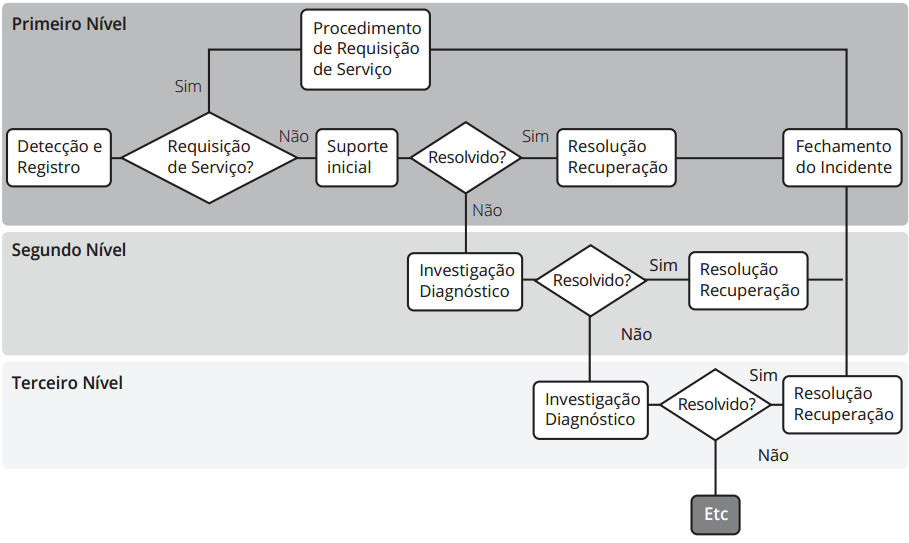
\includegraphics[width=15cm]{itil_images/gerenciamento_de_incidentes.png}
\label{figura:Gerenciamento de incidentes retirado do ITIL v3 Fundation}
\end{figure}

\subparagraph*{Conceitos}
\begin{itemize}[noitemsep]
	\item {\bfseries Prazos para execução e escalonamento (Timescales)} \\
		Prazos de execução precisam ser acordados para todos os estágios de tratamento ao inci-
		dente (que irão diferir de acordo com a prioridade do incidente)

	\item {\bfseries Modelos de Incidente (Incident Models) } \\
		Um modelo de incidente é uma forma de pré-definir os passos que devem ser seguidos
		para manusear um incidente, de maneira acordada. Define os passos a serem executados, a
		ordem cronológica dos passos, responsabilidades, tempos de execução, procedimentos de
		escalonamento e geração de evidências.

\end{itemize}


\subparagraph{Gerenciamento de Problema}
Uma forma de reduzir a quantidade de incidentes é evitando a sua recorrência. Através q
do processo de Gerenciamento de Problema, os problemas com causas não identificadas
serão analisados e corrigidos para que não voltem a acontecer.
É importante que o processo de Gerenciamento de Problema venha acompanhado do
Gerenciamento de Mudança, fazendo com que a correção dos erros seja previamente
analisada em relação aos riscos. Muitas vezes a correção de um erro acaba gerando mais
incidentes e criando impacto para os usuários.

Este processo tem como missão minimizar a interrupção nos serviços de TI através da orga-
nização dos recursos para solucionar problemas de acordo com as necessidades de negócio,
prevenindo a recorrência dos mesmos e registrando informações que melhorem a maneira
pela qual a organização de TI trata os problemas, resultando em níveis mais altos de disponibilidade e produtividade.

\begin{figure}[!h]
\caption{Gerenciamento de problema retirado do ITIL v3 Fundation}
\centering % para centralizarmos a figura
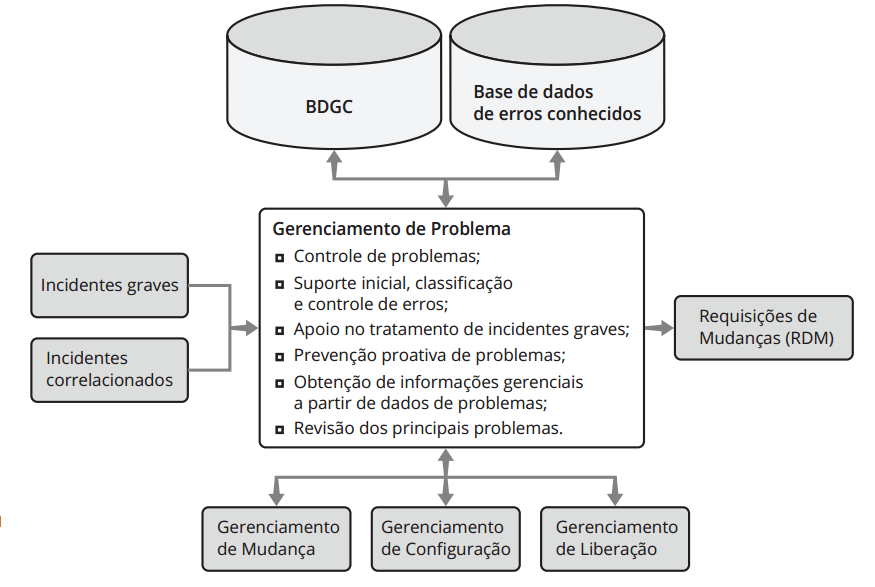
\includegraphics[width=15cm]{itil_images/gerenciamento_de_problema.png}
\label{figura:Gerenciamento de problemas retirado do ITIL v3 Fundation}
\end{figure}

\subparagraph*{Conceitos}
\begin{itemize}[noitemsep]
	\item {\bfseries Modelos de Problemas (Problem Models)} \\
		Muitos problemas são únicos e devem receber tratamento individual. Porém, alguns incidentes 				podem ocorrer novamente por causa de problemas adormecidos ou camuflados.
	\item {\bfseries Base de Dados de Erros Conhecidos (Know Error Database) } \\
		O propósito dessa base de dados é permitir o armazenamento de conhecimentos prévios a
	respeito de incidentes e problemas (e como eles foram superados), possibilitando assim o
	diagnóstico e resolução rápidos. O registro de erros conhecidos deve conter todos os detalhes da 		falha ocorrida e seus respectivos sintomas, juntamente com detalhes de qualquer solução de contorno 		que venha a ser realizada para solucionar incidentes ou problemas.
\end{itemize}





\subparagraph{Gerenciamento de acesso}

Este processo ajuda a organização a manter a confidencialidade das suas informações de
forma mais efetiva. O Gerenciamento da Segurança da Informação define as políticas de
segurança, enquanto o Gerenciamento de Acesso executa o que foi definido a partir destas
políticas, sendo assim uma parte operacional da segurança da informação.
Concede ao usuário o direito de usar um serviço, mas nega o acesso a usuários não autorizados.

\begin{figure}[!h]
\caption{Gerenciamento de acesso retirado do ITIL v3 Fundation}
\centering % para centralizarmos a figura
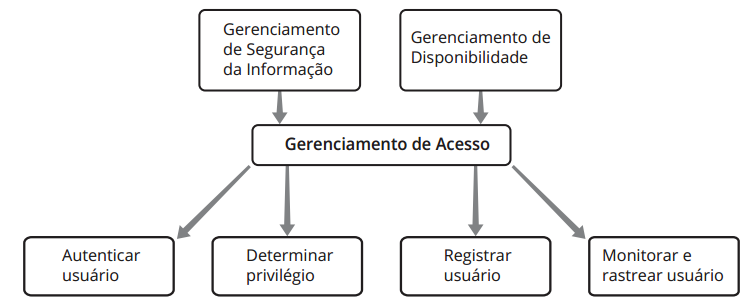
\includegraphics[width=15cm]{itil_images/gerenciamento_de_acesso.png}
\label{figura:Gerenciamento de acesso retirado do ITIL v3 Fundation}
\end{figure}

\subparagraph*{Conceitos}
Gerenciamento de Acesso está fundamentado nos conceitos listados abaixo
\begin{itemize}[noitemsep]
	\item {\bfseries Acesso (Access) }
		Refere-se ao nível e extensão da funcionalidade de um serviço ou dado permitido a um usuário.
	\item {\bfseries Identidade (Identity) }
		Refere-se à informação sobre o usuário, que o distingue dos demais e demonstra sua situação 				dentro da organização.
	\item {\bfseries  Direitos ou Privilégios (Rights) }
		Referem-se à regulamentação definida, que determina o acesso a ser oferecido ao usuário
		para um serviço ou grupos de serviços.
\end{itemize}





\subparagraph{Execução de requisição}
O termo Execução de Requisição é usado como uma descrição genérica para muitos tipos de demandas colocadas sobre a área de TI por seus usuários (Requisição de Serviço).
Muitas delas são na verdade pequenas mudanças de baixo risco, ocorrendo com frequência.



\begin{figure}[!h]
\caption{Execução de requisição do ITIL v3 Fundation}
\centering % para centralizarmos a figura
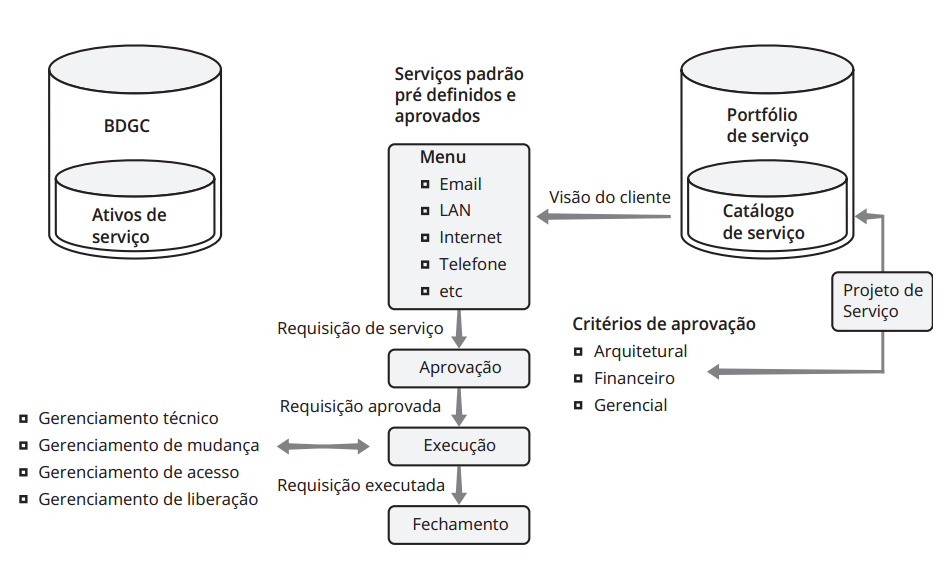
\includegraphics[width=15cm]{itil_images/execucao_de_requisicao.png}
\label{figura:Execução de requisiçao retirado do ITIL v3 Fundation}
\end{figure}




\subparagraph*{Conceitos}
Solicitações de serviço ocorrem frequentemente e requerem seu atendimento através de
uma maneira consistente, de forma a atender os níveis de servidos acordados. Para dar
assistência a essas solicitações, muitas organizações criam Modelos de Requisições (Request
Models) pré-definidos, os quais tipicamente incluem alguma forma de pré-aprovação por
parte do processo de Gerenciamento de Mudança.

\section{ Melhoria de processo (TO - BE)}

\begin{itemize}[noitemsep]
	\item Gestão de Conhecimento e Auto-Ajuda
	\item	Para base de conhecimento, será preciso incluir
	\begin{itemize}[noitemsep]
		\item Manual para suporte dos usuários
		\item Documentação completa dos produtos de software
		\item Documentação de Problemas comuns
		\item Base de dados de erros e suas workarounds
		\item Base de dados de improvement sugestions
	\end{itemize}
	A base de conhecimento será lançada como uma extensão do
	suporte web page
	\item Monitoramento de performace
\end{itemize}




\subsection{Propostas de modelagem}
\subsubsection{Atendimento de requisição }
\begin{figure}[!h]
\caption{Gerencia de requisição}
\centering % para centralizarmos a figura
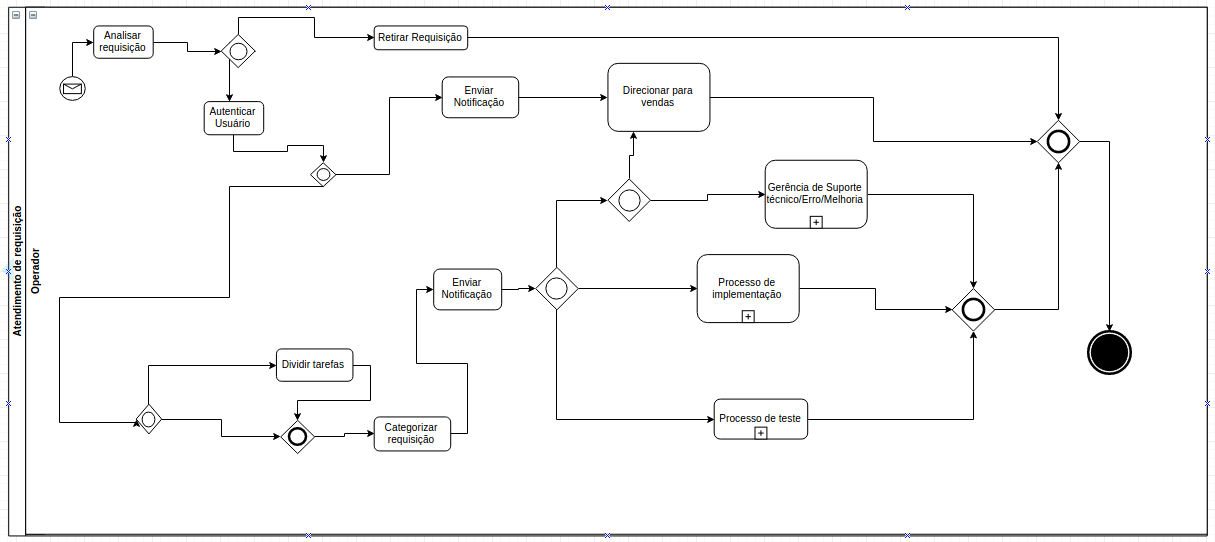
\includegraphics[width=15cm]{to_be/01_atendimento_de_requisicao.png}
\label{figura:atendimento_requisicao_to_be}
\end{figure}

Como primeira ação foi necessário achar os indicadores chave de performace,
onde foi possivel mapear o relacionamento desses indicadores chave com os fatores
\cite{cartlidge2007introductory} criticos de sucesso

\subsubsection{Atendimento técnico}
\begin{figure}[!h]
\caption{Atendimento técnico}
\centering % para centralizarmos a figura
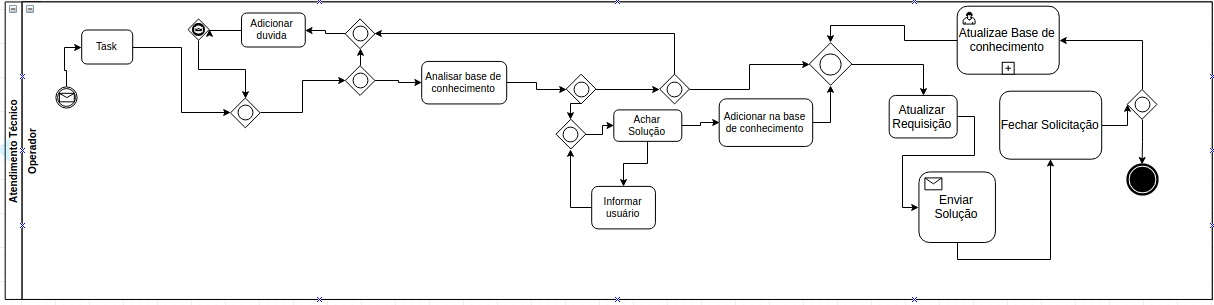
\includegraphics[width=15cm]{to_be/02_atendimento_tecnico.png}
\label{figura:suporte_tecnico_to_be}
\end{figure}



\subsubsection{Atendimento para erro no sistema}

\begin{figure}[!h]
\caption{Atendimento para erro no sistema}
\centering % para centralizarmos a figura
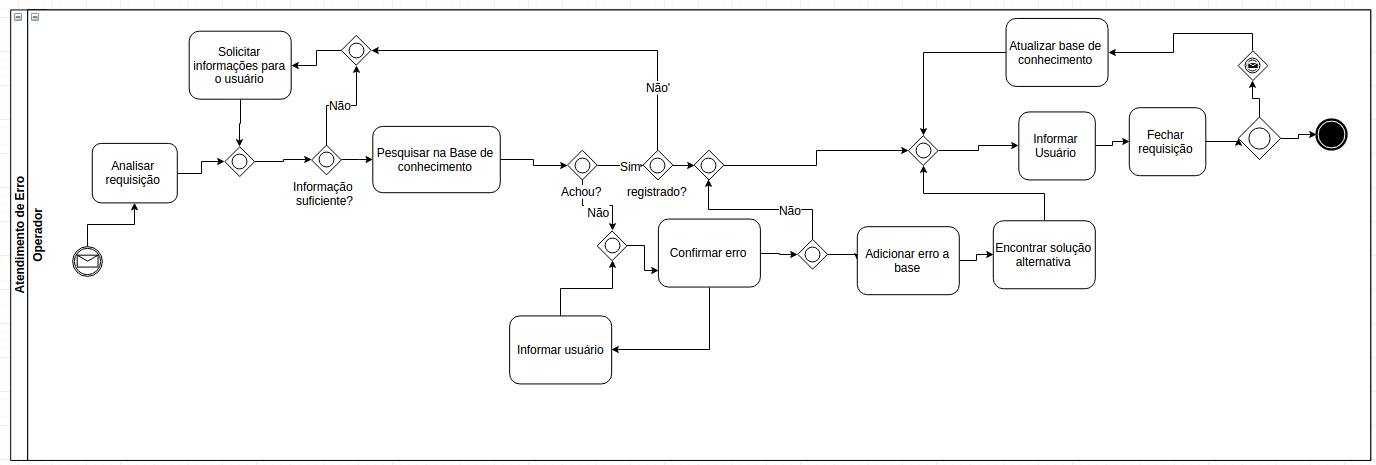
\includegraphics[width=15cm]{to_be/03_atendimento_de_erro.png}
\label{figura:atendimento_de_erro_to_be}
\end{figure}


\bibliographystyle{ieeetr}
\bibliography{./ref}



\appendix
\begin{appendices}

%\begin{landscape}% Landscape page



\section{ Comparação entre as modelagens}

\subsection{Comparação atendimento de requisição}
\begin{figure}[!h]
\caption{Gerencia de requisição - AS-IS}
\centering % para centralizarmos a figura
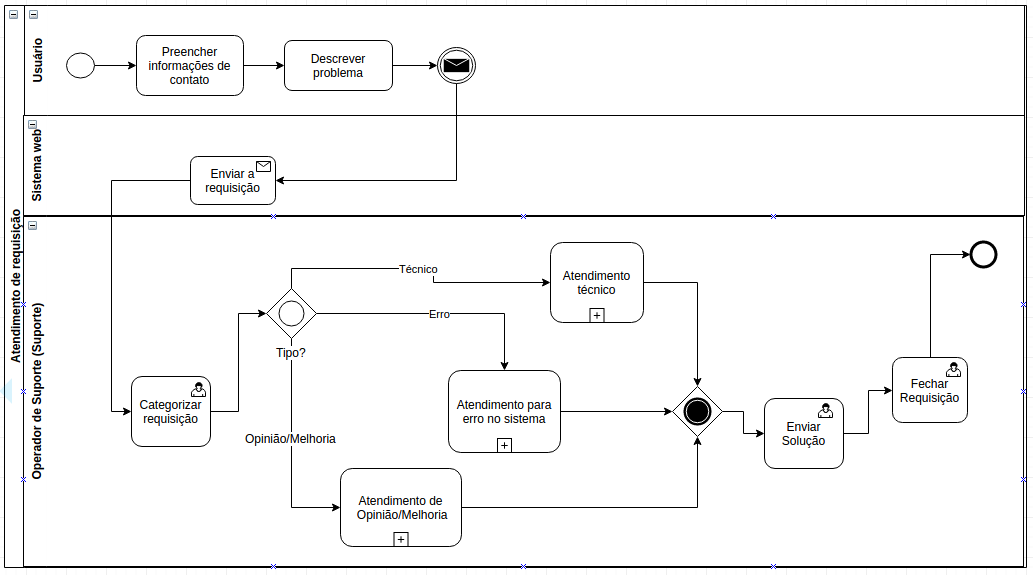
\includegraphics[width=15cm,height=6cm]{as-is/01_atendimento_de_requisicao.png}
\label{figura:atendimento_requisicao_as_is}
\end{figure}


\begin{figure}[!h]
\caption{Gerencia de requisição- TO-BE}
\centering % para centralizarmos a figura
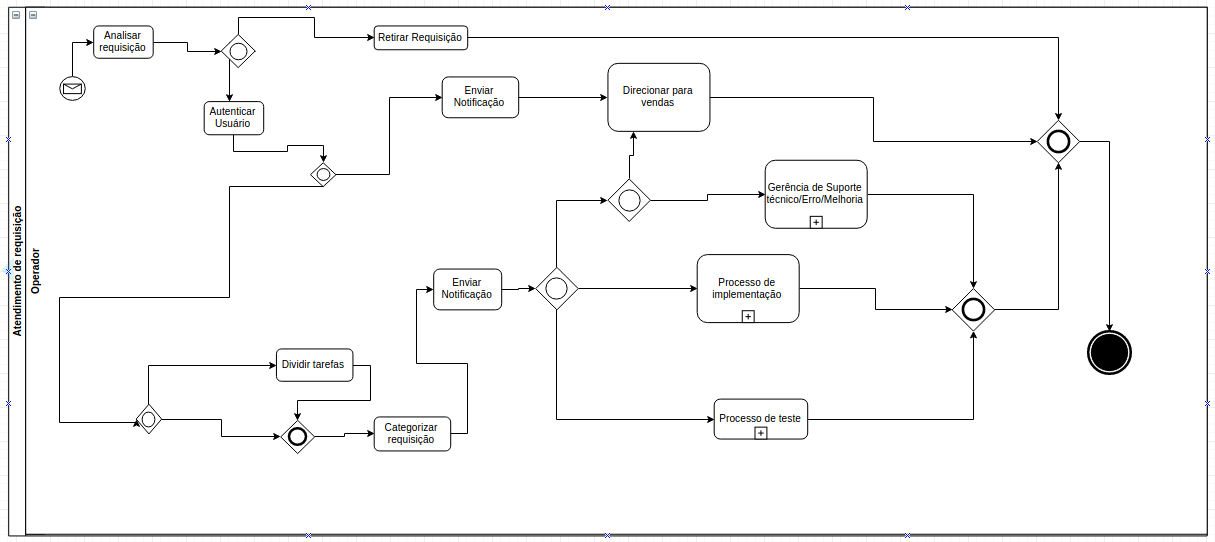
\includegraphics[width=16cm,height=7cm]{to_be/01_atendimento_de_requisicao.png}
\label{figura:atendimento_requisicao_to_be}
\end{figure}

\clearpage

\subsection{Comparação atendimento técnico}

\begin{figure}[!h]
\caption{Atendimento técnico - AS-IS}
\centering % para centralizarmos a figura
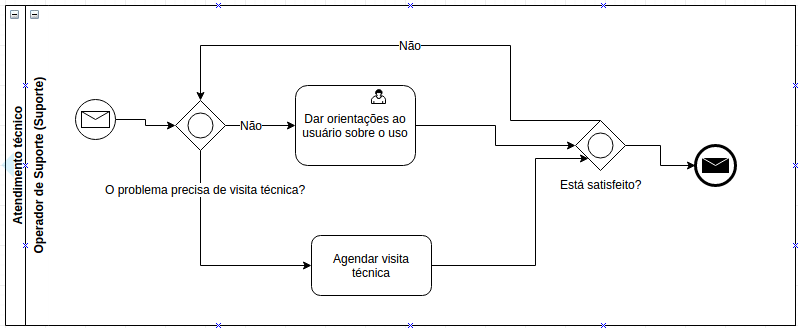
\includegraphics[width=15cm]{as-is/02_atendimento_tecnico.png}
\label{figura:suporte_tecnico_as_is}
\end{figure}

\begin{figure}[!h]
\caption{Atendimento técnico - TO-BE}
\centering % para centralizarmos a figura
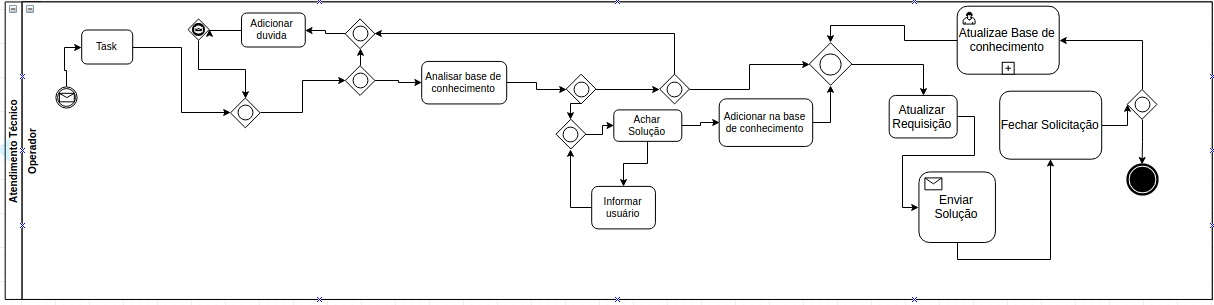
\includegraphics[width=16cm,height=7cm]{to_be/02_atendimento_tecnico.png}
\label{figura:suporte_tecnico_to_be}
\end{figure}

\clearpage
\subsection{Comparação atendimento para erro no sistema}

\begin{figure}[!h]
\caption{Atendimento para erro no sistema - AS-IS}
\centering % para centralizarmos a figura
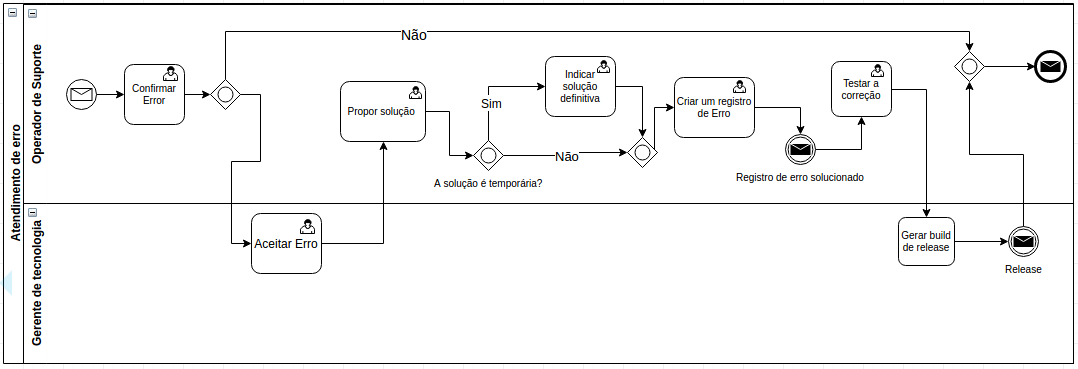
\includegraphics[width=16cm, height=7cm]{as-is/03_atendimento_de_erro.png}
\label{figura:atendimento_de_erro_as_is}
\end{figure}


\begin{figure}[!h]
\caption{Atendimento para erro no sistema - TO-BE}
\centering % para centralizarmos a figura
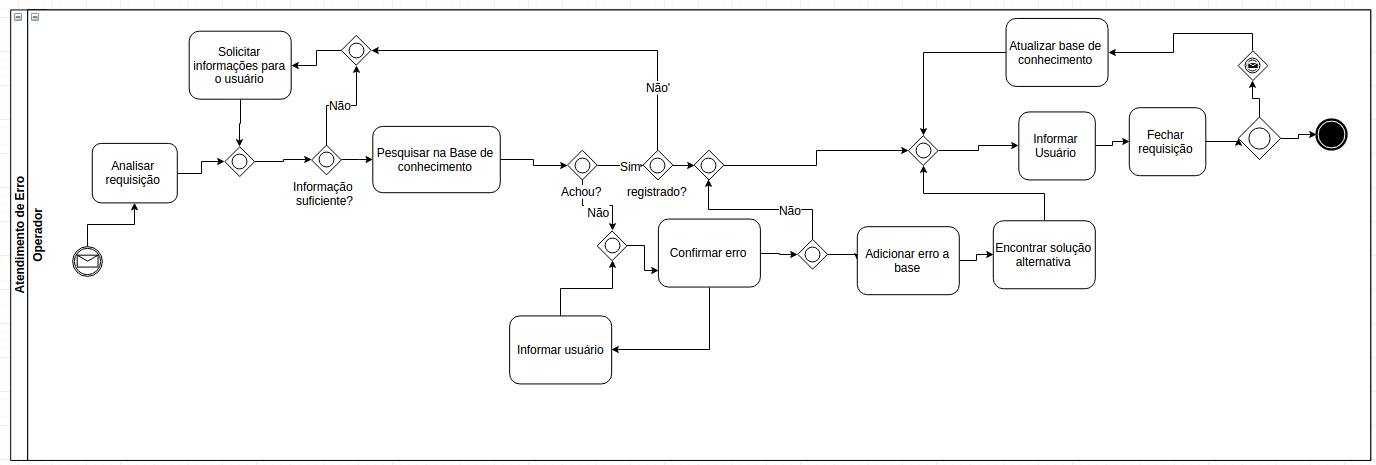
\includegraphics[width=16cm,height=7cm]{to_be/03_atendimento_de_erro.png}
\label{figura:atendimento_de_erro_to_be}
\end{figure}

\clearpage% Flush page


\subsection{Comparação Atendimento de Opinião/Melhoria}

\begin{figure}[!h]
\caption{Atendimento de Opinião/Melhoria - AS-IS}
\centering % para centralizarmos a figura
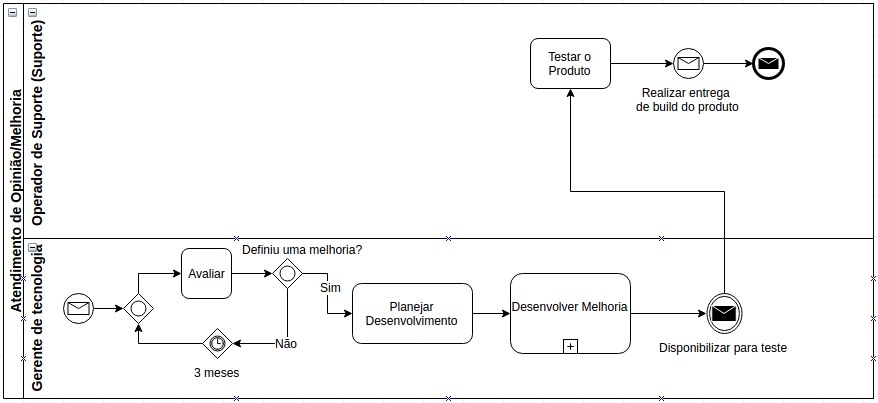
\includegraphics[width=15cm,height=7cm]{as-is/04_atendimento_de_melhoria.png}
\label{figura:atendimento_de_melhoria_as_is}
\end{figure}

\begin{figure}[!h]
\caption{Atendimento para erro no sistema -  TO-BE}
\centering % para centralizarmos a figura
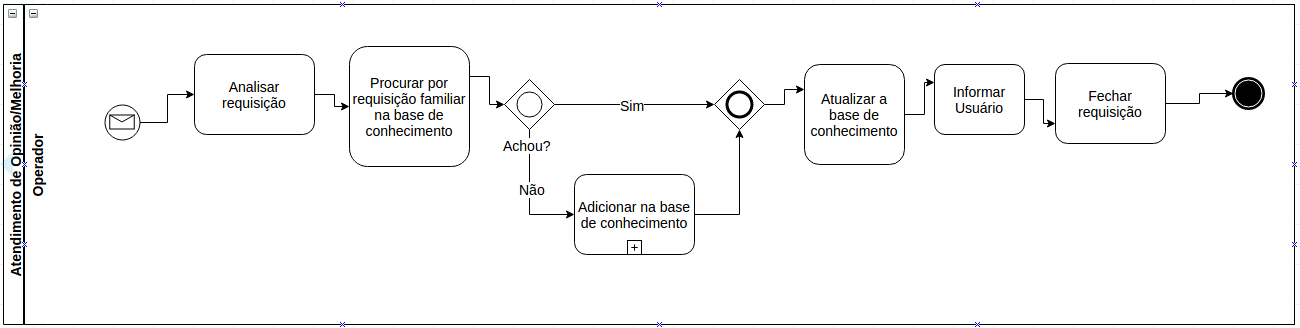
\includegraphics[width=15cm,height=7cm]{to_be/04_atendimento_de_melhoria.png}
\label{figura:atendimento_de_erro_to_be}
\end{figure}

\clearpage
\section{Pesquisa de satisfação}

Durante o decorrer do projeto, foi
realizada uma pesquisa de satisfação do
cliente. Foi solicitados aos clientes
responder a algumas perguntas sobre sua
satisfação com o suporte ao usuário. Um total de
60 clientes, que entraram em contato com um suporte
nos últimos doze meses, receberam o questionário, mas
apenas 3 devolveram. Segue o formulário utilizado na
pesquisa de satisfação. Esse formulário também
poderá ser usado como pesquisa de satisfação como descrito no
tópico de monitoramento de perfomace proposto no TO-BE


\begin{table}[htb]
\centering
\caption{Questões de Pesquisa sobre suporte ao usuário}
\label{my-label}
\begin{tabular}{cl|c|c|c|c|}
\cline{3-6}
\multicolumn{1}{l}{}                              &                              & \cellcolor[HTML]{9AFF99}                                     & \cellcolor[HTML]{9AFF99}                               & \cellcolor[HTML]{9AFF99}                                 & \cellcolor[HTML]{9AFF99}                                 \\ \cline{1-2}
\multicolumn{2}{|c|}{\cellcolor[HTML]{FFFC9E}\textbf{Suporte ao Usuário}}        & \multirow{-2}{*}{\cellcolor[HTML]{9AFF99}\textbf{Excelente}} & \multirow{-2}{*}{\cellcolor[HTML]{9AFF99}\textbf{Bom}} & \multirow{-2}{*}{\cellcolor[HTML]{9AFF99}\textbf{Fraco}} & \multirow{-2}{*}{\cellcolor[HTML]{9AFF99}\textbf{Pobre}} \\ \hline
\multicolumn{2}{|c|}{\cellcolor[HTML]{FFFFC7}Impressão geral}                    &                                                              &                                                        &                                                          &                                                          \\ \hline
\multicolumn{2}{|c|}{\cellcolor[HTML]{FFFFC7}Tempo de resposta}                  &                                                              &                                                        &                                                          &                                                          \\ \hline
\multicolumn{2}{|c|}{\cellcolor[HTML]{FFFFC7}Competência técnica dos operadores} &                                                              &                                                        &                                                          &                                                          \\ \hline
\multicolumn{2}{|c|}{\cellcolor[HTML]{FFFFC7}Estilo de comunicação}              &                                                              &                                                        &                                                          &                                                          \\ \hline
\end{tabular}
\end{table}


% Please add the following required packages to your document preamble:
% \usepackage{multirow}
% \usepackage[table,xcdraw]{xcolor}
% If you use beamer only pass "xcolor=table" option, i.e. \documentclass[xcolor=table]{beamer}
\begin{table}[htb]
\centering
\caption{Questões sobre a sugestão de melhoria}
\label{my-label}
\begin{tabular}{cl|c|c|c|c|}
\cline{3-6}
\multicolumn{1}{l}{}                           &                            & \cellcolor[HTML]{9AFF99}                                     & \cellcolor[HTML]{9AFF99}                               & \cellcolor[HTML]{9AFF99}                                 & \cellcolor[HTML]{9AFF99}                                 \\ \cline{1-2}
\multicolumn{2}{|c|}{\cellcolor[HTML]{FFFC9E}\textbf{Sugestão de Melhoria}} & \multirow{-2}{*}{\cellcolor[HTML]{9AFF99}\textbf{Excelente}} & \multirow{-2}{*}{\cellcolor[HTML]{9AFF99}\textbf{Bom}} & \multirow{-2}{*}{\cellcolor[HTML]{9AFF99}\textbf{Fraco}} & \multirow{-2}{*}{\cellcolor[HTML]{9AFF99}\textbf{Pobre}} \\ \hline
\multicolumn{2}{|c|}{\cellcolor[HTML]{FFFFC7}Qualidade das soluções}        &                                                              &                                                        &                                                          &                                                          \\ \hline
\multicolumn{2}{|c|}{\cellcolor[HTML]{FFFFC7}Tempo de resolução}            &                                                              &                                                        &                                                          &                                                          \\ \hline
\multicolumn{2}{|c|}{\cellcolor[HTML]{FFFFC7}Feedback}                      &                                                              &                                                        &                                                          &                                                          \\ \hline
\end{tabular}
\end{table}


% Please add the following required packages to your document preamble:
% \usepackage{multirow}
% \usepackage[table,xcdraw]{xcolor}
% If you use beamer only pass "xcolor=table" option, i.e. \documentclass[xcolor=table]{beamer}
% Please add the following required packages to your document preamble:
% \usepackage{multirow}
% \usepackage[table,xcdraw]{xcolor}
% If you use beamer only pass "xcolor=table" option, i.e. \documentclass[xcolor=table]{beamer}
\begin{table}[htb]
\centering
\caption{Questões dobre reporte de erros}
\label{my-label}
\begin{tabular}{cl|c|c|c|c|}
\cline{3-6}
\multicolumn{1}{l}{}                              &                              & \cellcolor[HTML]{9AFF99}                                     & \cellcolor[HTML]{9AFF99}                               & \cellcolor[HTML]{9AFF99}                                 & \cellcolor[HTML]{9AFF99}                                 \\ \cline{1-2}
\multicolumn{2}{|c|}{\cellcolor[HTML]{FFFC9E}\textbf{Reporte de erros}}          & \multirow{-2}{*}{\cellcolor[HTML]{9AFF99}\textbf{Excelente}} & \multirow{-2}{*}{\cellcolor[HTML]{9AFF99}\textbf{Bom}} & \multirow{-2}{*}{\cellcolor[HTML]{9AFF99}\textbf{Fraco}} & \multirow{-2}{*}{\cellcolor[HTML]{9AFF99}\textbf{Pobre}} \\ \hline
\multicolumn{2}{|c|}{\cellcolor[HTML]{FFFFC7}Qualidade da solução dos erros}     &                                                              &                                                        &                                                          &                                                          \\ \hline
\multicolumn{2}{|c|}{\cellcolor[HTML]{FFFFC7}Tempo de resolução}                 &                                                              &                                                        &                                                          &                                                          \\ \hline
\multicolumn{2}{|c|}{\cellcolor[HTML]{FFFFC7}Competência técnica dos operadores} &                                                              &                                                        &                                                          &                                                          \\ \hline
\end{tabular}
\end{table}

\end{appendices}


\end{document}
